

\tikzset{every picture/.style={line width=0.75pt}} %set default line width to 0.75pt        

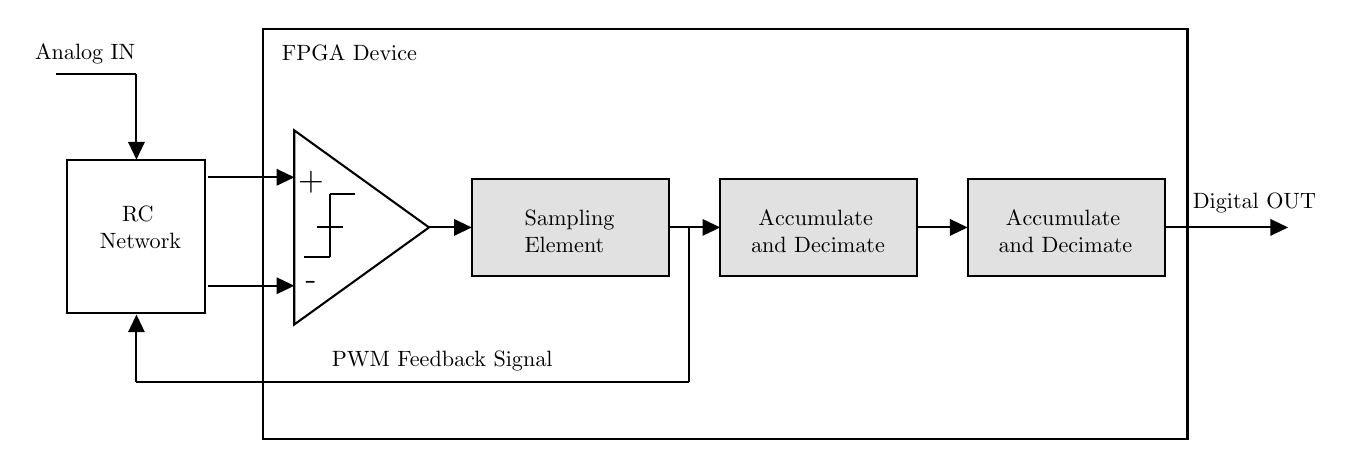
\begin{tikzpicture}[x=0.75pt,y=0.75pt,yscale=-0.95,xscale=0.95]
%uncomment if require: \path (0,300); %set diagram left start at 0, and has height of 300

%Shape: Rectangle [id:dp9604023161903008] 
\draw   (124.05,6.64) -- (593.05,6.64) -- (593.05,214.64) -- (124.05,214.64) -- cycle ;
%Straight Lines [id:da9484599770004658] 
\draw    (330.44,107.42) -- (353.05,107.42) ;
\draw [shift={(356.05,107.42)}, rotate = 180] [fill={rgb, 255:red, 0; green, 0; blue, 0 }  ][line width=0.08]  [draw opacity=0] (8.93,-4.29) -- (0,0) -- (8.93,4.29) -- cycle    ;

%Shape: Rectangle [id:dp7904328314933544] 
\draw  [fill={rgb, 255:red, 225; green, 225; blue, 225 }  ,fill opacity=1 ] (230,82.9) -- (330.05,82.9) -- (330.05,131.94) -- (230,131.94) -- cycle ;

%Straight Lines [id:da4819176246297532] 
\draw    (208.39,107.42) -- (227.05,107.42) ;
\draw [shift={(230.05,107.42)}, rotate = 180] [fill={rgb, 255:red, 0; green, 0; blue, 0 }  ][line width=0.08]  [draw opacity=0] (8.93,-4.29) -- (0,0) -- (8.93,4.29) -- cycle    ;

%Straight Lines [id:da24497687439569482] 
\draw    (60,70) -- (60,29.64) ;

\draw [shift={(60,73)}, rotate = 270] [fill={rgb, 255:red, 0; green, 0; blue, 0 }  ][line width=0.08]  [draw opacity=0] (8.93,-4.29) -- (0,0) -- (8.93,4.29) -- cycle    ;
%Straight Lines [id:da9302636844153138] 
\draw    (137.05,137) -- (96.05,137) ;

\draw [shift={(140.05,137)}, rotate = 180] [fill={rgb, 255:red, 0; green, 0; blue, 0 }  ][line width=0.08]  [draw opacity=0] (8.93,-4.29) -- (0,0) -- (8.93,4.29) -- cycle    ;
%Straight Lines [id:da2916048291189839] 
\draw    (137.05,82) -- (96.05,82) ;

\draw [shift={(140.05,82)}, rotate = 180] [fill={rgb, 255:red, 0; green, 0; blue, 0 }  ][line width=0.08]  [draw opacity=0] (8.93,-4.29) -- (0,0) -- (8.93,4.29) -- cycle    ;
%Shape: Triangle [id:dp8965603701252123] 
\draw   (208.39,107.42) -- (140.05,156.64) -- (140.05,58.2) -- cycle ;
%Shape: Rectangle [id:dp2519733387539336] 
\draw  [fill={rgb, 255:red, 225; green, 225; blue, 225 }  ,fill opacity=1 ] (356,82.9) -- (456.05,82.9) -- (456.05,131.94) -- (356,131.94) -- cycle ;

%Straight Lines [id:da7883255728251393] 
\draw    (456.44,107.42) -- (478.52,107.42) ;
\draw [shift={(481.52,107.42)}, rotate = 180] [fill={rgb, 255:red, 0; green, 0; blue, 0 }  ][line width=0.08]  [draw opacity=0] (8.93,-4.29) -- (0,0) -- (8.93,4.29) -- cycle    ;

%Shape: Rectangle [id:dp34966320633084025] 
\draw  [fill={rgb, 255:red, 225; green, 225; blue, 225 }  ,fill opacity=1 ] (481.5,82.9) -- (581.55,82.9) -- (581.55,131.94) -- (481.5,131.94) -- cycle ;

%Shape: Rectangle [id:dp20202629131702943] 
\draw   (25,73) -- (95,73) -- (95,150.64) -- (25,150.64) -- cycle ;
%Straight Lines [id:da3350824826473666] 
\draw    (19.05,29.64) -- (60,29.64) ;


%Straight Lines [id:da8160728779847974] 
\draw    (582.05,107.42) -- (641.05,107.42) ;
\draw [shift={(644.05,107.42)}, rotate = 180] [fill={rgb, 255:red, 0; green, 0; blue, 0 }  ][line width=0.08]  [draw opacity=0] (8.93,-4.29) -- (0,0) -- (8.93,4.29) -- cycle    ;

%Straight Lines [id:da4116203957240303] 
\draw    (158.05,90.27) -- (158.05,122.64) ;


%Straight Lines [id:da2244964116397019] 
\draw    (145.05,122.64) -- (158.05,122.64) ;


%Straight Lines [id:da41850801552553585] 
\draw    (158.05,90.27) -- (171.05,90.27) ;


%Straight Lines [id:da28517286500051164] 
\draw    (151.71,107.42) -- (164.71,107.42) ;


%Straight Lines [id:da7677560417405613] 
\draw    (60,154.64) -- (60,185.64) ;

\draw [shift={(60,151.64)}, rotate = 90] [fill={rgb, 255:red, 0; green, 0; blue, 0 }  ][line width=0.08]  [draw opacity=0] (8.93,-4.29) -- (0,0) -- (8.93,4.29) -- cycle    ;
%Straight Lines [id:da2763081409638619] 
\draw    (340.24,107.42) -- (340.24,185.64) ;


%Straight Lines [id:da4366815569167197] 
\draw    (340.24,185.64) -- (60,185.64) ;



% Text Node
\draw (62.05,107.42) node  [scale=0.8] [align=left] { \ \ \ RC \\Network};
% Text Node
\draw (215.05,175.14) node  [scale=0.8] [align=left] {PWM Feedback Signal};
% Text Node
\draw (168.05,19) node  [scale=0.8] [align=left] {FPGA Device};
% Text Node
\draw (279.66,109.27) node  [scale=0.8] [align=left] {Sampling\\ Element};
% Text Node
\draw (405.66,109.27) node  [scale=0.8] [align=left] { \ Accumulate\\and Decimate};
% Text Node
\draw (531.16,109.27) node  [scale=0.8] [align=left] { \ Accumulate\\and Decimate};
% Text Node
\draw (34,19.42) node  [scale=0.8] [align=left] {Analog IN};
% Text Node
\draw (627,95.05) node  [scale=0.8] [align=left] {Digital OUT};
% Text Node
\draw (148.55,84.55) node  [scale=1.2] [align=left] {+};
% Text Node
\draw (148.55,135.14) node   [align=left] {{\large -}};


\end{tikzpicture}
